%%% LaTeX Template: Article/Thesis/etc. with colored headings and special fonts
%%%
%%% Source: http://www.howtotex.com/
%%% Feel free to distribute this template, but please keep to referal to http://www.howtotex.com/ here.
%%% February 2011
%%%
%%% Modified October 2015 by CDM

%%%  Preamble
\documentclass[11pt,letterpaper]{article}
\usepackage[margin=1.0in]{geometry}
\usepackage[T1]{fontenc}
\usepackage[bitstream-charter]{mathdesign}
\usepackage[latin1]{inputenc}					
\usepackage{amsmath}						
\usepackage{xcolor}
\usepackage{cite}
\usepackage{hyphenat}
\usepackage{graphicx}
\usepackage{float}
\usepackage{subfigure}
\usepackage{sectsty}
\usepackage[compact]{titlesec} 
\usepackage[tablegrid]{vhistory}
\usepackage{pbox}
\allsectionsfont{\color{accentcolor}\scshape\selectfont}

%%% Definitions
\definecolor{accentcolor}{rgb}{0.0,0.0,0.5} 
\newcommand{\teamname}{Eyeronic}
\newcommand{\productname}{Eye Tracker}
\newcommand{\coursename}{CSE 4316: Senior Design I}
\newcommand{\semester}{Fall 2015}
\newcommand{\docname}{Architectural Design Specification}
\newcommand{\department}{Department of Computer Science \& Engineering}
\newcommand{\university}{The University of Texas at Arlington}
\newcommand{\authors}{Krishna Bhattarai \\ James Stone \\ Fernando Do Nascimento \\ Joseph Trinh \\ Zachary Allen}

%%% Headers and footers
\usepackage{fancyhdr}
	\pagestyle{fancy}						% Enabling the custom headers/footers
\usepackage{lastpage}	
	% Header (empty)
	\lhead{}
	\chead{}
	\rhead{}
	% Footer
	\lfoot{\footnotesize \teamname \ - \semester}
	\cfoot{}
	\rfoot{\footnotesize page \thepage\ of \pageref{LastPage}}	% "Page 1 of 2"
	\renewcommand{\headrulewidth}{0.0pt}
	\renewcommand{\footrulewidth}{0.4pt}

%%% Change the abstract environment
\usepackage[runin]{abstract}			% runin option for a run-in title
%\setlength\absleftindent{30pt}			% left margin
%\setlength\absrightindent{30pt}		% right margin
\abslabeldelim{\quad}	
\setlength{\abstitleskip}{-10pt}
\renewcommand{\abstractname}{}
\renewcommand{\abstracttextfont}{\color{accentcolor} \small \slshape}	% slanted text

%%% Start of the document
\begin{document}

%%% Cover sheet
{\centering \huge \color{accentcolor} \sc \textbf{\department \\ \university} \par}
\vspace{1 in}
{\centering \huge \color{accentcolor} \sc \textbf{\docname \\ \coursename \\ \semester} \par}
\vspace{0.5 in}
\begin{figure}[h!]
	\centering
   	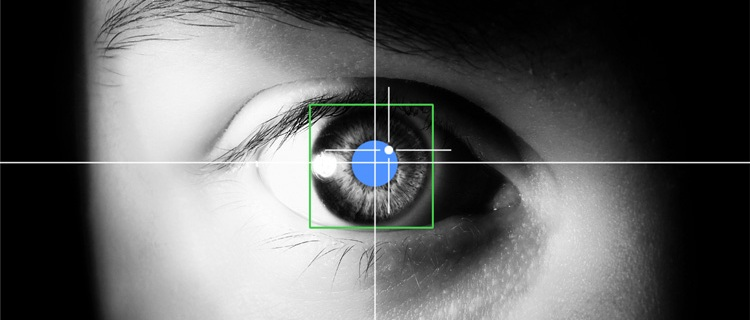
\includegraphics[width=0.60\textwidth]{images/eyetracker.jpg}
\end{figure}
\vspace{0.5 in}
{\centering \huge \color{accentcolor} \sc \textbf{\teamname \\ \productname} \par}
\vspace{0.5 in}
{\centering \large \sc \textbf{\authors} \par}
\newpage


%\vspace{1 in}
%\centerline{January 13th, 2012}
%\newpage

%%% Revision History
\begin{versionhistory}
  	\vhEntry{0.1}{11.18.2015}{KM | JS | ZA | FN | JT}{Created Document}
  	%\vhEntry{0.2}{10.05.2015}{AT|GH}{complete draft}
  	%\vhEntry{0.3}{10.12.2015}{AT|GH}{release candidate 1}
  	%\vhEntry{1.0}{10.20.2015}{AT|GH|CB}{official release}
  	%\vhEntry{1.1}{10.31.2015}{AL}{added design review requests}
\end{versionhistory}
\newpage

%%% Table of contents
\setcounter{tocdepth}{2}
\tableofcontents
\newpage

%%% List of figures and tables (optional)
\listoffigures
\listoftables
\newpage

\section{Introduction}
%Your introduction should describe your product concept in sufficient detail that the architectural design will be easy to follow. The introduction may include information used in the first sections of your SRS for this purpose. At a minimum, ensure that the product concept, scope and key requirements are described

This product shall have three layers that work in unison to track the pupil of the user. The three layers in our system are the Software layer, Daughter Board, and the Jetson TK1. The three layers will be discussed more in the following sections.
\newpage
\section{System Overview}
%This section should describe the overall structure of your software system. Think of it as the strategy for how you will build the system. An architectural "layer" is the top-level logical view, or an abstraction, of your design. Layers should be composed of related elements of similar capabilities, and should be highly independent of other layers, but should have very clearly defined interfaces and interactions with other layers. Each layer should be identified individually and should be unique as to its function and purpose within the system. This section should also contain the high-level block diagram of the layers, as shown in the example below, as well as detailed descriptions of the functions of each layer.
The system consists of three major layers which are: The Daughter Board Layer, The Jetson TK1 Layer, and the Software Layer. The Daughter board is the main interface between the MIPI camera module and the Jetson TK1. It contains the OmniVision 5640 sensor that interfaces to the Jetson TK1.
The Jetson TK1 layer provides the interface between the MIPI camera and the USB. This layer is what communicates with the computer and the Daughter board. It uses USB to power the device and transfer the data to a computer. 
The Software layer takes input from the Jetson Interface, processes that data, and tracks the pupil movement in real time. Various Computer Vision algorithms such as the Canny Edge Detector, Gaussian Smoothing, and the Random Sampling Consensus are implemented by the software layer to accurately track the pupil movement.



\begin{figure}[h!]
	\centering
 	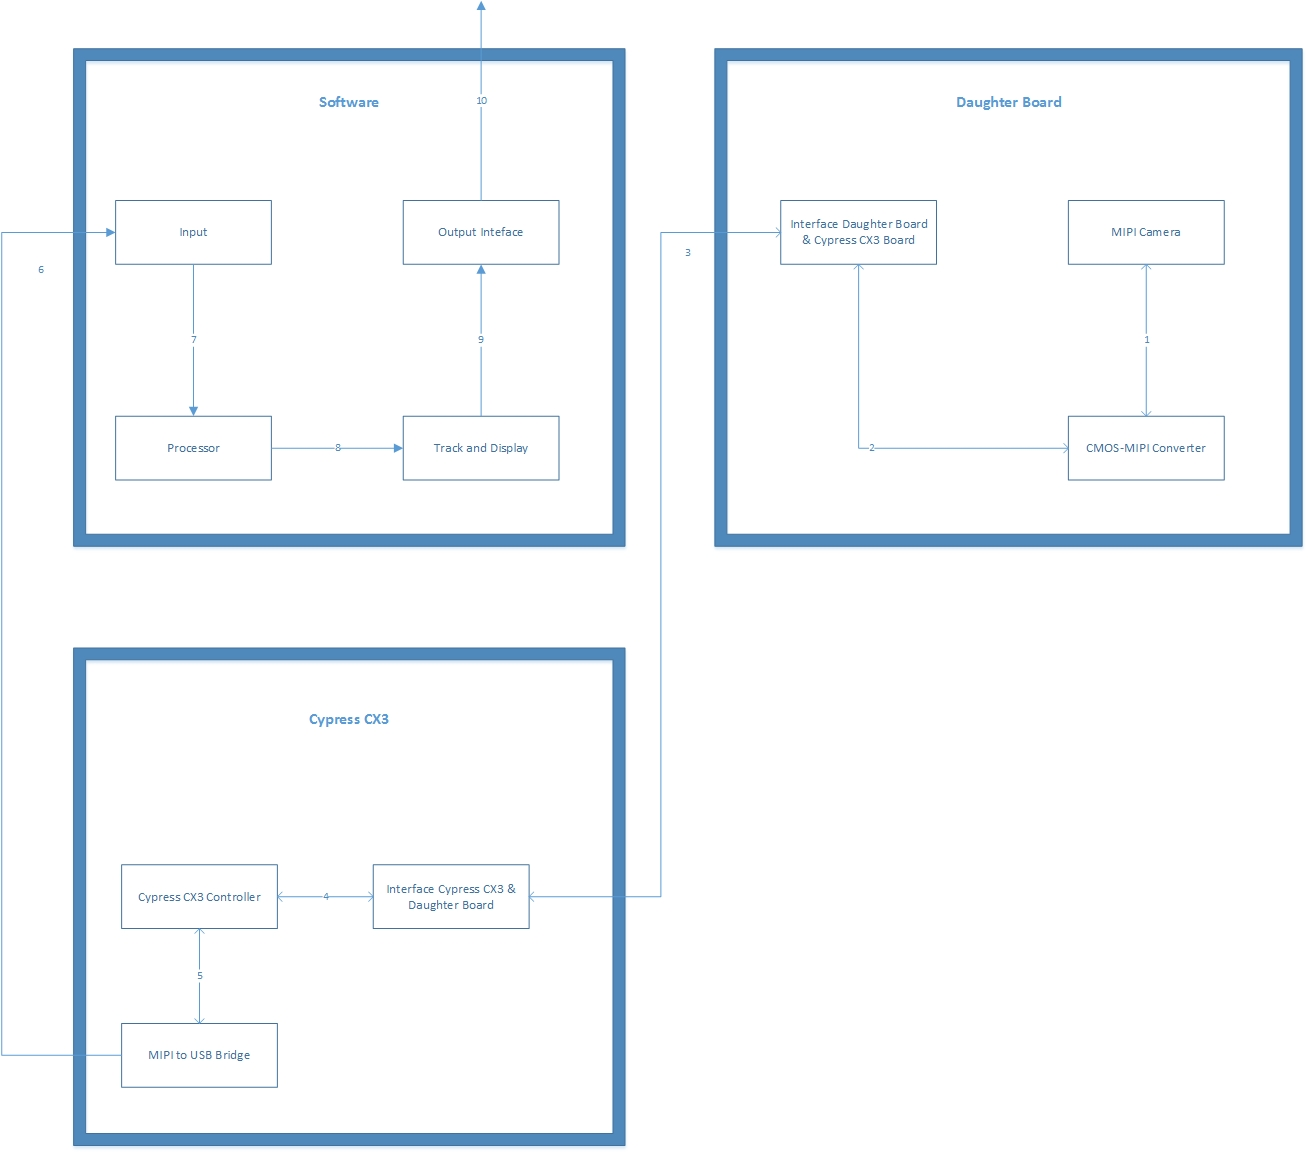
\includegraphics[width=0.60\textwidth]{images/Diagram_WHOLE.jpg}
 \caption{A simple architectural layer diagram}
\end{figure}

\subsection{Software Layer Description}
%Each layer should be described separately in detail. Descriptions should include the features, functions, critical interfaces and interactions of the layer. The description should clearly define the services that the layer provides. Also include any conventions that your team will use in describing the structure: naming conventions for layers, subsystems, modules, and data flows; interface specifications; how layers and subsystems are defined; etc. 
The software layer makes use of the OpenCV library and implements the entire program in C++ language. It consists of three major subsystems. The first subsystem is the Input subsystem. It gets input from the interface provided by the Jetson TK1. A video stream from a device (or a disk for test purposes) is read and stored into a CV::Mat structure. This structure will later be passed onto the processing subsystem.
The goal of the processing subsystem is to filter out all the noise (anything but the pupil) and it does so utilizing readily available OpenCV algorithms which shall be discussed in detail later in the document.
The final layer is the display layer which gathers information from the processor and displays the final result (fitted elipse) into the original video stream. 
\newline

\subsection{Daughter Board Description}
%Each layer should be described separately in detail. Descriptions should include the features, functions, critical interfaces and interactions of the layer. The description should clearly define the services that the layer provides. Also include any conventions that your team will use in describing the structure: naming conventions for layers, subsystems, modules, and data flows; interface specifications; how layers and subsystems are defined; etc. 
The daughter board is a board that is used to interface between the camera module 
and the Jetson TK1. This board uses a high-speed rugged ground plane socket 
(Base BRD Connector) to transfer the data that the camera captures to the TK1. In 
order for the camera module (pcDuino Camera Module) to function properly the 
daughter board needed a new camera connector, since the original connector is not 
compatible. We replaced the old connector with the Panasonic connector 
(AXK824145WG). The purpose of the new camera connector is to interface the 
camera with the Base BRD Connector. The daughter board contains the OmniVision 
5640 that is interfaced through the 2-lane MIPI interface.
\newline

\subsection{Jetson TK1 Description}
%Each layer should be described separately in detail. Descriptions should include the features, functions, critical interfaces and interactions of the layer. The description should clearly define the services that the layer provides. Also include any conventions that your team will use in describing the structure: naming conventions for layers, subsystems, modules, and data flows; interface specifications; how layers and subsystems are defined; etc. 
The Jetson TK1 is a MIPI to USB interface. This controller is fully functional with 
any image sensor that is compliant with a MIPI Camera Serial Interface (OmniVision 
5640). The Jetson TK1 is used to control the communication between a computer 
and the device, since it uses a USB connection to power the device and transfer the 
data that it collected. Also in order for the device to store the data read from the 
camera module, it uses EEPROMS in order to prevent loosing data in cases the 
device looses power. Then the device will transfer its data to the computer via USB. 
The Jetson TK1 is also connected to the MIPI camera.

\newpage
\section{Subsystem Definitions \& Data Flow}
%This section breaks down your layer abstraction to another level of detail. Here you grapically represent the logical subsytems that compose each layer and show the interactions/interfaces between those subsystems. A subsystem can be thought of as a programming unit that implements one of the major functions of the layer. It, therefore, has data elements that serve as source/sinks for other subsystems. The logical data elements that flow between subsystems need to be explicitly defined at this point, beginning with a data flow-like diagram based on the block diagram.
The following section shows a high level diagram of all layers of our system.
\begin{figure}[h!]
	\centering
 	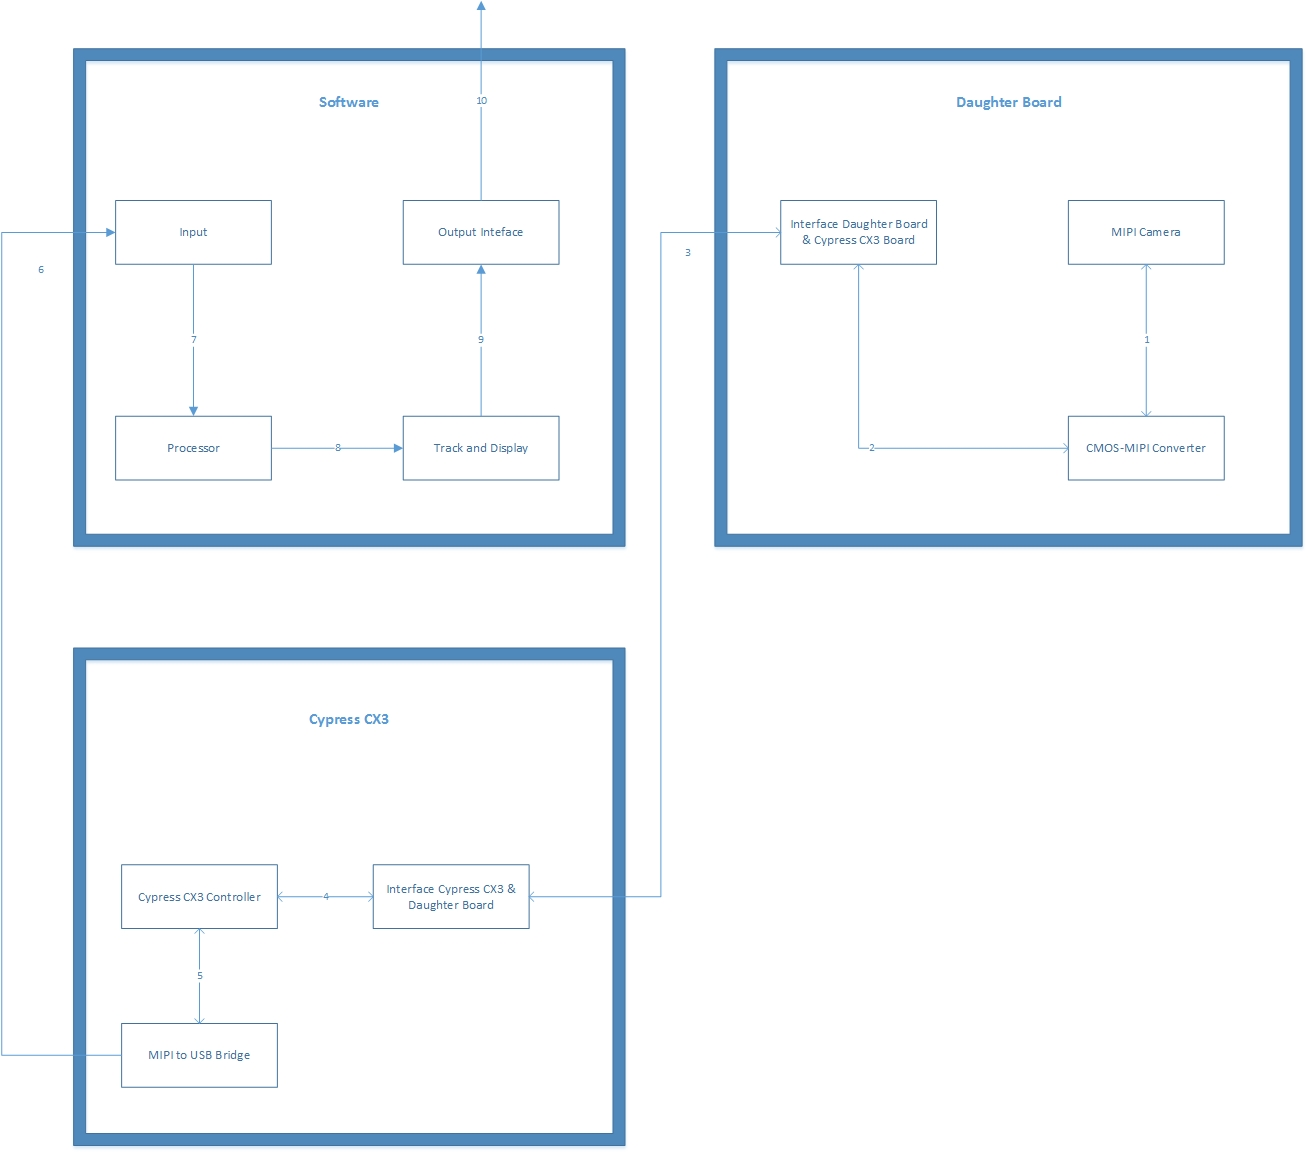
\includegraphics[width=\textwidth]{images/Diagram_WHOLE.jpg}
 \caption{A simple data flow diagram}
\end{figure}

\newpage
\section{Software Subsystems}
The Raspberry Pi 3 is a single-board computer that accepts MIPI cameras. This device will be used to connect an infrared MIPI Camera and stream a live video fee from the camera via ethernet. In order to avoid connectivity issues with the Jetson TK-1, the Raspberry Pi 3 has been configured with a static IP address. To assure that the live video fee has a small latency, the Raspberry Pi 3 will be connected to a router. The video feed is being streaming using VLC. 

%%%Change Pictures
\begin{figure}[h!]
	\centering
 	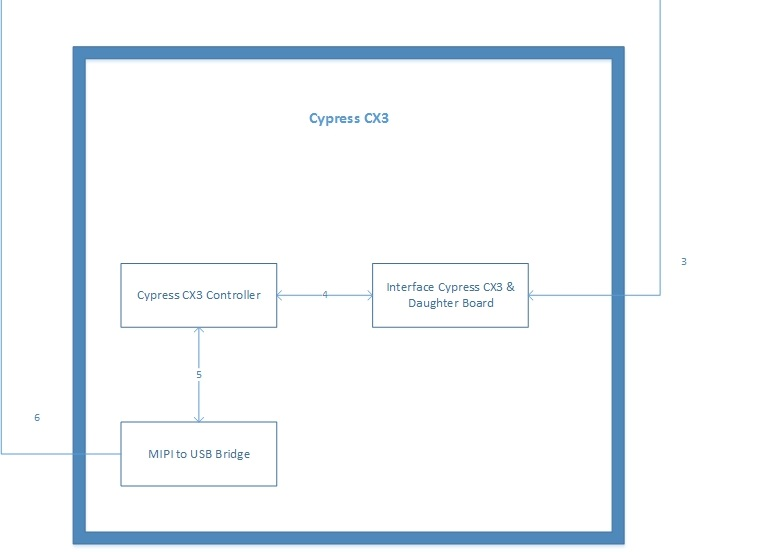
\includegraphics[width=0.60\textwidth]{images/Cypress}
 \caption{Jetson Subsystem Diagram}
\end{figure}


\subsection{Central Processing Unit}
The CPU of the Raspberry Pi is connected to multiple components. One of those components is the camera connector that needs to have a 15 pin ribbon cable in order to accurately receive a video feed from the MIPI camera. In this product, the camera connector is connected to an HDMI Extension Board via a ribbon cable. The CPU of this device also sends the live video fee using VLC via ethernet. All the user needs to have to capture the live video feed is the static IP address of the Raspberry Pi 3. 

%%%Update Imagei
\begin{figure}[h!]
	\centering
 	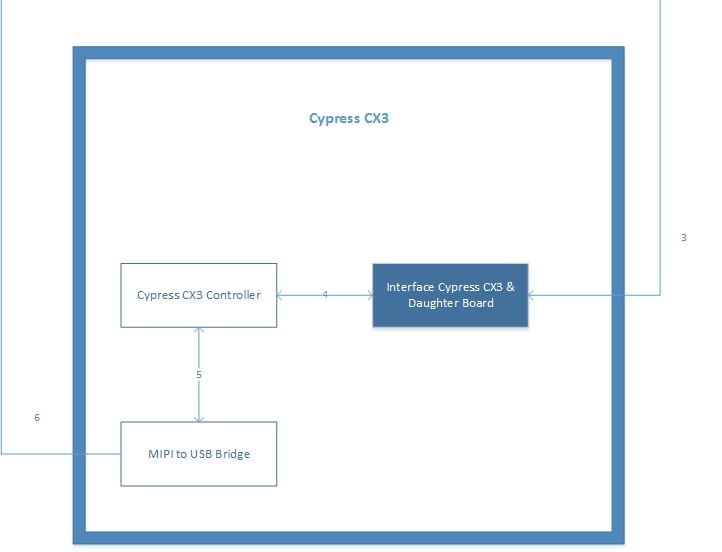
\includegraphics[width=0.60\textwidth]{images/Cypress_Interface}
 \caption{GPID Interface}
\end{figure}

\subsubsection{Assumptions}
The user knows how to connect to the Raspberry Pi 3 via SSH using the Jetson TK-1 terminal.

\subsubsection{Responsibilities}
The responsibility of the Raspberry Pi 3 CPU is to start the live video stream.

\subsubsection{Subsystem Interfaces}

\begin{table}[H]
\caption {Central Processing Unit}
\begin{center}
	\begin{tabular}{ | p{1cm} | p{6cm} | p{3cm} | p{3cm} |}
	\hline
	ID & Description & Inputs & Outputs \\ \hline
	\#01 & HDMI Extension Board & \pbox{3cm}{Input 1 - MIPI Data} & \pbox{3cm}{Output 1 - MIPI Power \\ Output 2 - MIPI Clock} \\ \hline
	\#02 & Ethernet Connector & \pbox{3cm}{Input 1 - RX D2+ \\ Input 2 - RX D2- \\Input 3 - BI D3+ \\ Input 4 - BI D3- \\ Input 5 - BI D4+ \\Input 6 - BI D4-} & \pbox{3cm}{Output 1 - RX D2+ \\ Output 2 - RX D2- \\ Output 3 - BI D3+ \\ Output 4 - BI D3- \\ Output 5 - BI D4+ \\ Output 6 - BI D4-} \\ \hline
	\end{tabular}
\end{center}
\end{table}

\subsection{HDMI Extension Board}
The sole purpose of the HDMI Extension Board is to give the user a longer distance between the MIPI camera and Raspberry Pi 3 in order to make the device more comfortable to the user. The HDMI Extension Board consists of two identical boards that are connected with an HDMI cable. One of the boards is connected via a ribbon cable to the Raspberry Pi 3 while the other board is connected to the Arducam Spy Camera for Raspberry Pi. The HDMI cable is used to send and receive data from and to the Raspberry Pi 3.

%%Update Picture + Caption
\begin{figure}[h!]
	\centering
	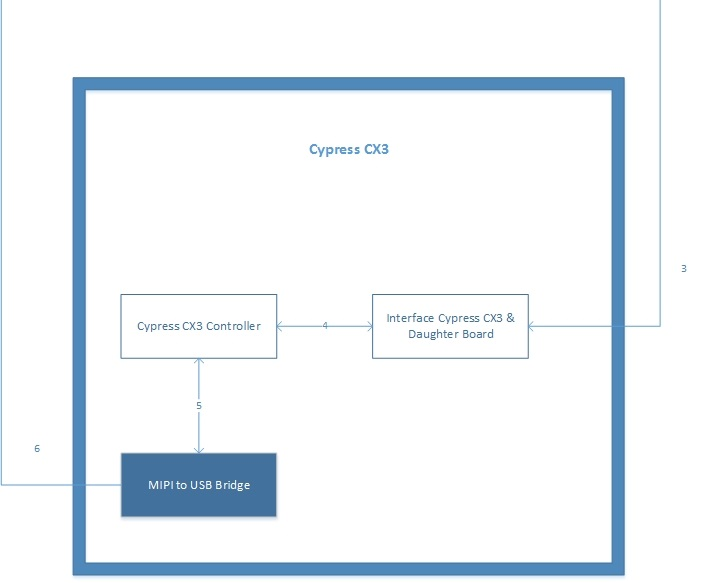
\includegraphics[width=0.60\textwidth]{images/Cypress_MIPI}
	\caption{MIPI to USB Subsystem}
\end{figure}

\subsubsection{Assumptions}
The HDMI cable connected between both boards is fully functional and compatible with both boards.

\subsubsection{Responsibilities}
The HDMI Extension Boards are responsible with interfacing the infrared MIPI camera and the Raspberry Pi 3, and capture and sending a video feed.

\subsubsection{Subsystem Interfaces}
\begin{table}[H]
\caption{HDMI Extension Board}
\begin{center}
	\begin{tabular}{ | p{1cm} | p{6cm} | p{3cm} | p{3cm} |}
	\hline
	ID & Description & Inputs & Outputs \\ \hline
	\#03 & Board Connected To Raspberry Pi 3 & \pbox{3cm}{Input 1 - 3.3V \\ Input 2 - GND \\ Input 3 - LVDS Data 0 to 1 +/- \\ Input 4 - LVDS CLK +/-} & \pbox{3cm}{Output 1 - 3.3V \\ Output 2 - GND \\ Output 3 - LVDS Data 0 to 1 +/- \\ Output 4 - LVDS CLK +/-} \\ \hline
	\#04 & Both HDMI Extension Boards Connected Together & \pbox{3cm}{Input 1 - 3.3V \\ Input 2 - GND \\ Input 3 - LVDS Data 0 to 1 +/- \\ Input 4 - LVDS CLK +/-} & \pbox{3cm}{Output 1 - 3.3V \\ Output 2 - GND \\ Output 3 - LVDS Data 0 to 1 +/- \\ Output 4 - LVDS CLK +/-} \\ \hline
	\#05 & HDMI Extension Board to MIPI Camera & \pbox{3cm}{Input 1 - MIPI Data 0 to 1 +/- \\ Input 2 - MIPI CLK +/-} & \pbox{3cm}{Output 1 - 3.3V \\ Output 2 - GND \\ Output 3 - LVDS Data 0 to 1 +/- \\ Output 4 - LVDS CLK +/-} \\ \hline
	\end{tabular}
\end{center}
\end{table} 


\subsection{CMOS}
The Arducam Sensor Spy Camera for Raspberry Pi has an Omnivision OV5647 sensor in which the CMOS memory chip is used to convert the data collected from the camera into RAW RGB that a computer can use to manipulate the data.

%Update Picture
\begin{figure}[h!]
	\centering
	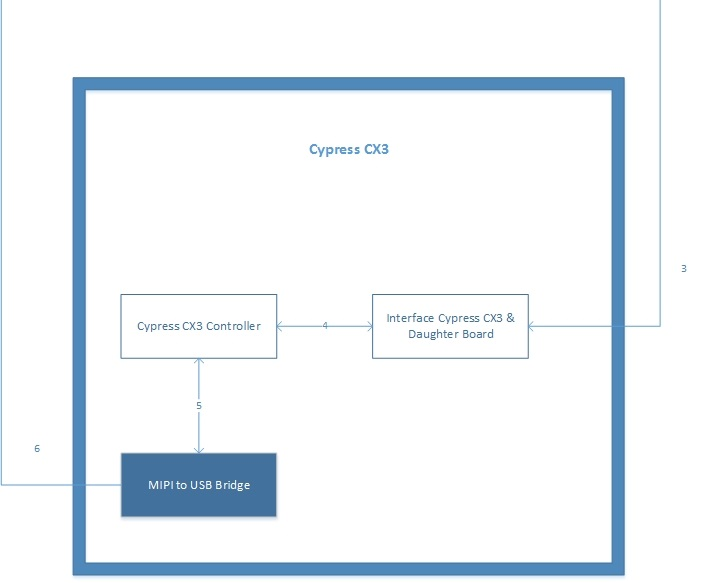
\includegraphics[width=0.60\textwidth]{images/Cypress_MIPI}
	\caption{MIPI to CMOS Conversion \& CMOS-HDMI Data Transfer}
\end{figure} 

\subsubsection{Assumptions}
The CMOS sensor on the MIPI camera is fully functional and has not been damaged during the removal of the infrared filter.

\subsubsection{Responsibilities}
The CMOS sensor converts the images captured from the MIPI camera to a RAW RGB format that can be used by the software to track the user's eye.

\subsubsection{Subsystem Interface}

\begin{table}[H]
\caption{CMOS Sensor OV5647}
\begin{center}
	\begin{tabular}{ | p{1cm} | p{6cm} | p{3cm} | p{3cm} |}
	\hline
	ID & Description & Inputs & Outputs \\ \hline
	\#06 & CMOS to HDMI & \pbox{3cm}{Input 1 - CLK +/-} & \pbox{3cm}{Output 1 - MIPI Data 0 to 1 +/-} \\ \hline
	\#07 & CMOS to MIPI & \pbox{3cm}{Input 1 - MIPI Data 0 to 1 +/-} & \pbox{3cm}{Output - CLK +/-} \\ \hline 
	\end{tabular}
\end{center}
\end{table}

\subsection{MIPI Camera}
The Arducam Sensor Spy Camera for Raspberry Pi is the camera that has been selected to work on this project. Other cameras that are compatible with Raspberry Pi may also work on the eye tracker system. The only modification that needs to be made to this camera is to remove the infrared filter from the camera.

%%%Update Pictures
\begin{figure}[h!]
	\centering
	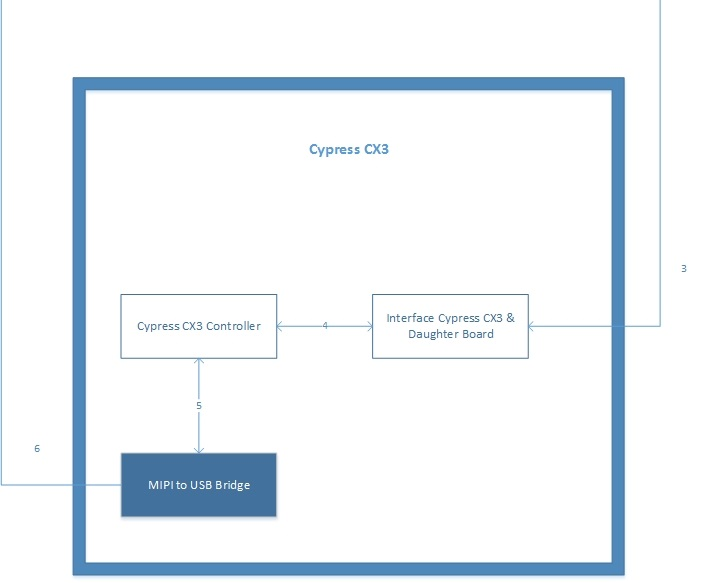
\includegraphics[width=0.60\textwidth]{images/Cypress_MIPI}
	\caption{MIPI to HDMI Connection \& MIPI to CMOS Connection}
\end{figure}

\subsubsection{Assumptions}
The camera used in the project is fully compatible with the Raspberry Pi 3, the camera has not been damaged during the infrared filter removal, and an infrared pass filter has been placed between the lens and the CMOS sensor.

\subsubsection{Responsibilities}
The responsibility of the MIPI Camera is to capture infrared video and send it to the Raspberry Pi in order to stream the video via ethernet.

\begin{table}[H]
\caption{MIPI Infrared Camera}
\begin{center}
	\begin{tabular}{ | p{1cm} | p{6cm} | p{3cm} | p{3cm} |}
	\hline
	ID & Description & Inputs & Outputs \\ \hline
	\#08 & MIPI to HDMI & \pbox{3cm}{Input 1 - 3.3V \\ Input 2 - GND} & \pbox{3cm}{} \\ \hline
	\#09 & MIPI to CMOS & \pbox{3cm}{Input 1 - MIPI Data 0 to 1 +/- \\ Input 2 - MIPI CLK +/-} & \pbox{3cm}{Output 1 - MIPI Data 0 to 1 +/-} \\ \hline
	\end{tabular}
\end{center}
\end{table} 

\newpage
\section{Daughterboard Subsystems}

\begin{figure}[h!]
	\centering
 	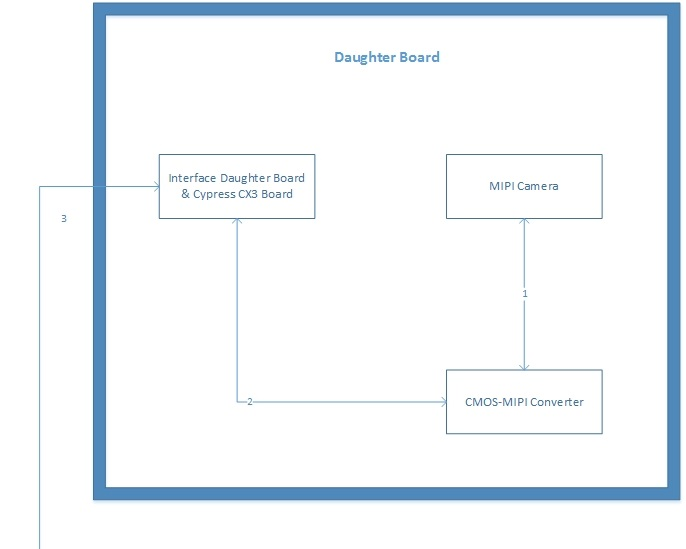
\includegraphics[width=0.60\textwidth]{images/DaughterBoard}
 \caption{Jetson TK-1 Diagram}
\end{figure}

\subsection{}

\subsection{GPID Interface}
The BRD is the interface between the Daughter board and Motherboard.

\begin{figure}[h!]
	\centering
 	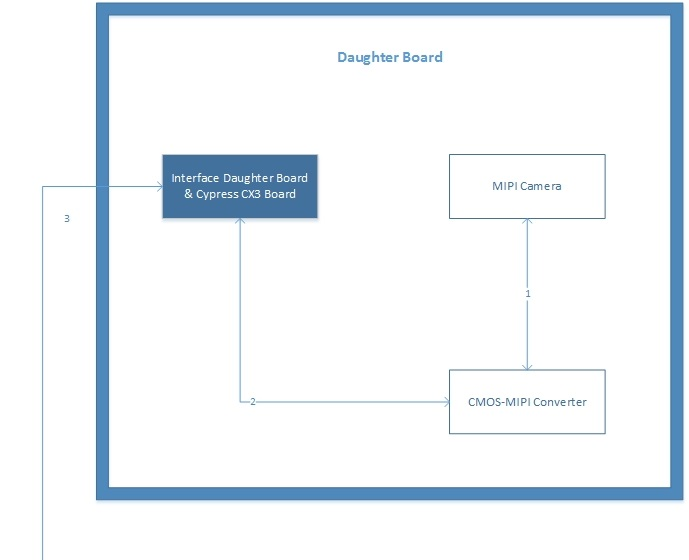
\includegraphics[width=0.60\textwidth]{images/DaughterBoard_Interface}
 \caption{GPID Interface}
\end{figure}

\subsubsection{Assumptions}
The BRD should communicate without any issues (like a BUS connection).

\subsubsection{Responsibilities}
The Base BRD Connector is used to interface between the daughter board and the MIPI Camera BRD Connector on the Jetson TK1 Board and vice versa.

\subsubsection{Subsystem Interfaces}
This connector contains 52 pins, but not all of the pins will be used. This connector is directly connected to the camera module connector in order to transfer the data back and forth at a faster rate.  Throughout this connector, multiple pins receive different types of voltages in order to perform different tasks. For complexity issues, the Base BRD Connector will be connected to the bottom layer of the Daughter Board.

\begin {table}[H]
\caption {GPID Interface}
\begin{center}
    \begin{tabular}{ | p{1cm} | p{6cm} | p{3cm} | p{3cm} |}
    \hline
    ID & Description & Inputs & Outputs \\ \hline
     \#03 & MIPI Controls & \pbox{3cm}{Input 1 - SCL \\ Input 2 - SDA} & \pbox{3cm}{Output 1 - MIPI Data \\ Output 2 - MIPI Clock \\ Output 3 - MIPI Power \\ Output 4 - SDA}  \\ \hline
    \end{tabular}
\end{center}
\end{table}
\newline

\subsection{MIPI Camera}
The camera module used for the Eye Tracker system is a 5MP pcDuino camera that will be used to capture data for processing. The pcDuino camera uses the OV5640 image sensor.

\begin{figure}[h!]
	\centering
 	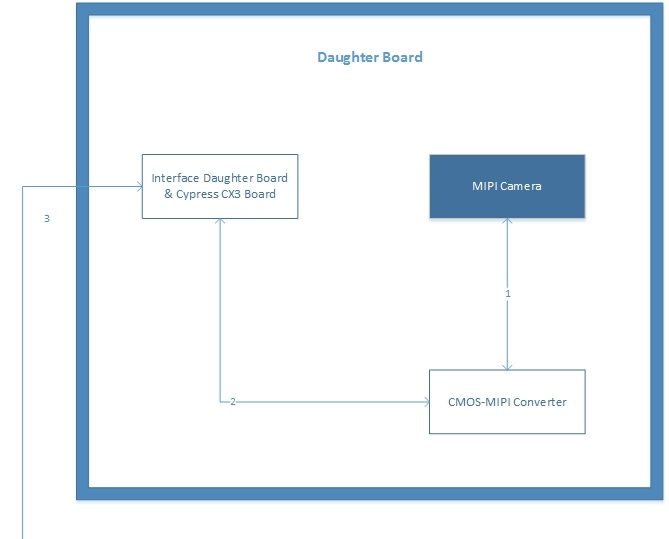
\includegraphics[width=0.60\textwidth]{images/DaughterBoard_Camera}
 \caption{Camera Module Diagram}
\end{figure}

\subsubsection{Assumptions}
The camera module will capture image and video at least 30FPS at 5MP.

\subsubsection{Responsibilities}
This image sensor is capable of capturing 2592x1944 active array of image and video at a minimum of 30 FPS. Since this new camera uses the OV5640, it is compatible with the Jetson TK1.

\subsubsection{Subsystem Interfaces}

The camera uses the OV5640 image sensor, which is a high quality CMOS image sensor.

\begin {table}[H]
\caption {MIPI Camera Interface}
\begin{center}
    \begin{tabular}{ | p{1cm} | p{6cm} | p{3cm} | p{3cm} |}
    \hline
    ID & Description & Inputs & Outputs \\ \hline
    \#01 & CMOS Data from Camera & \pbox{3cm}{Input 1 - SCL \\ Input 2 - SDA} & \pbox{3cm}{Output 1 - Data \\ Output 2 - Clock \\ Output 3 - SDA}  \\ \hline
    \end{tabular}
\end{center}
\end{table}
\newline

\subsection{CMOS-MIPI Converter}
The camera connector is new, and will be replacing the camera connector that was on the TK1 development board. The new connector allows for the use of the pcDuino camera module. This where the camera performs a CMOS to MIPI conversion in order to transfer the data collected from the camera module.

\begin{figure}[h!]
	\centering
 	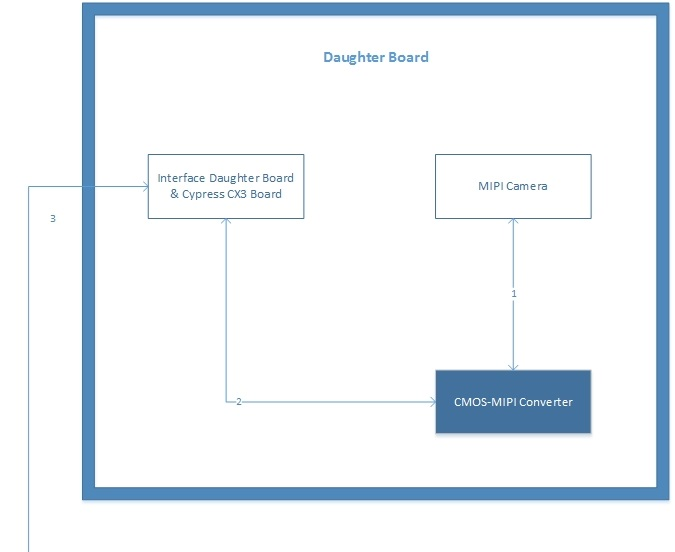
\includegraphics[width=0.60\textwidth]{images/DaughterBoard_converter}
 \caption{Camera Connector Diagram}
\end{figure}

\subsubsection{Assumptions}
The camera connector is compatible with the new module and the BRD.

\subsubsection{Responsibilities}
The camera connector is used to connect the camera module to the daughter board and transfer the data that the camera captures to the Base BRD Connector.

\subsubsection{Subsystem Interfaces}
In order for the camera module to function properly with the Jetson TK1, it received different voltage inputs in different pins. The datasheet of the OV5640 (Image Sensor) in order to determine which pins will be used on the camera connector and where to connect each pin at the Base BRD Connector. Since this camera will only be used for eye tracking purposes only, the user will not be able to reset the camera since we disabled the reset pin on the camera connector.

\begin {table}[H]
\caption {CMOS-MIPI Converter Interfaces}
\begin{center}
    \begin{tabular}{ | p{1cm} | p{6cm} | p{3cm} | p{3cm} |}
    \hline
    ID & Description & Inputs & Outputs \\ \hline
    \#02 & Camera Connector & \pbox{3cm}{Input 1 - MIPI Data \\ Input 2 - MIPI Clock \\ Input 3 - SDA} & \pbox{3cm}{Output 1 - Converted Data \\ Output 2 - Camera Clock Signal \\ Output 3 - SDA}  \\ \hline
    \end{tabular}
\end{center}
\end{table}

\newpage
\section{Cypress CX3 Subsystems}
%In this section, the layer is described in some detail in terms of its specific subsystems. Describe each of the layers and its subsystems in a separate chapter/major subsection of this document. The content of each subsystem description should be similar. Include in this section any special considerations and/or trade-offs considered for the approach you have chosen.%
This section discusses the software layer which consists of three major subsystems. 

\begin{figure}[h!]
	\centering
 	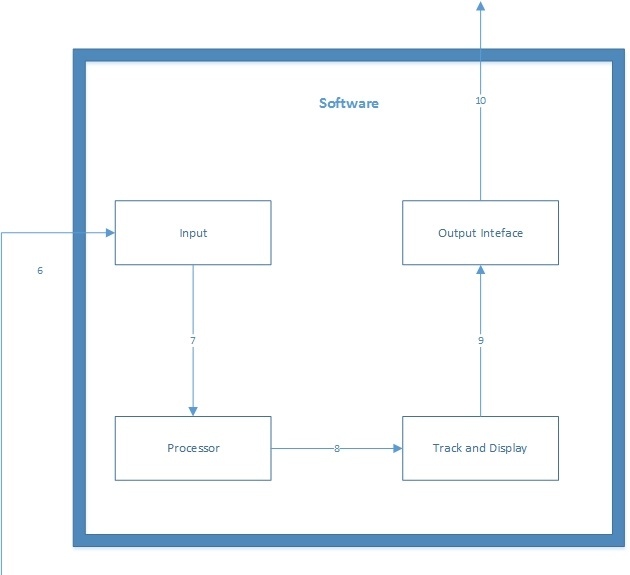
\includegraphics[width=0.60\textwidth]{images/Software.jpg}
 \caption{Software Subsystem}
\end{figure}

\subsection{Input Subsystem}
%This section should be a general description of a particular subsystem for the given layer. For most subsystems, an extract of the architectural block diagram with data flows is useful. This should consist of the subsystem being described and those subsystems with which it communicates.
The input subsystem is responsbile for receiving video input and sending it to the processing subsystem.

\begin{figure}[h!]
	\centering
 	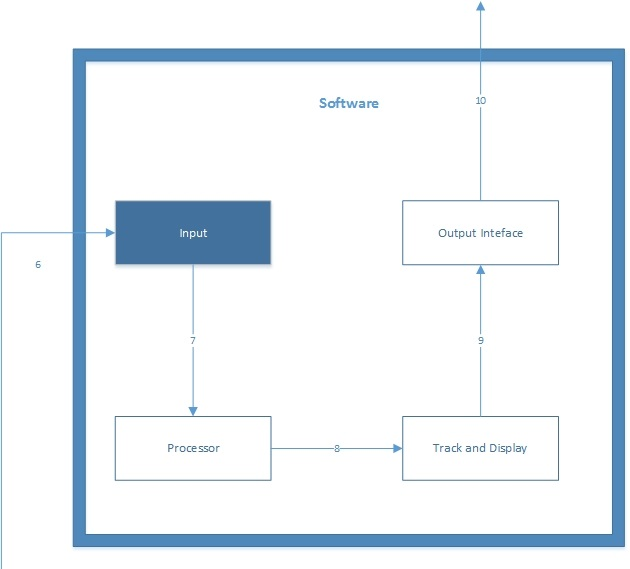
\includegraphics[width=0.60\textwidth]{images/Software_Input.jpg}
 \caption{Input Subsystem}
\end{figure}

\subsubsection{Assumptions}
%Any assumptions made in the definition of the subsystem should be listed and described. Pay particular attention to assumptions concerning interfaces and interactions with other layers.
We are assuming that we are getting the required video data from the Cypress CX3 or any other USB device. The software is flexible enough to be able to read the data from a file or directly from the hardware. 


\subsubsection{Responsibilities}
%Each of the responsibilities/features/functions/services of the subsystem as identified in the architectural summary must be expanded to more detailed responsibilities. These responsibilities form the basis for the identification of the finer-grained responsibilities of the layer's internal subsystems. Clearly describe what each subsystem does.
This subsystem is responsible for properly receiving the video data and sending it to the processor subsystem. 

\subsubsection{Subsystem Interfaces}
%Each of the inputs and outputs for the subsystem are defined here. Create a table with an entry for each labelled interface that connects to this subsystem. For each entry, describe any incoming and outgoing data elements will pass through this interface.
The input could either from a file (for test purposes) or a live stream from the cypress camera. The details are shown in the table. 


\begin {table}[H]
\caption {Input Subsystem Interface} 
\begin{center}
    \begin{tabular}{ | p{1cm} | p{6cm} | p{3cm} | p{3cm} |}
    \hline
    ID & Description & Inputs & Outputs \\ \hline
    \#06 & Receive video data & \pbox{3cm}{From Camera} & \pbox{3cm}{ Video data  }  \\ \hline
    %\#02 & Input video data from the File & \pbox{3cm}{N/A} & \pbox{3cm}{Video data}  \\ \hline
    \end{tabular}
\end{center}
\end{table}
\newline

\subsection{Processor Subsystem}
The processor subsystem takes in the video input, processes it sends the processed data to the Track and Display subsystem.

\begin{figure}[h!]
	\centering
 	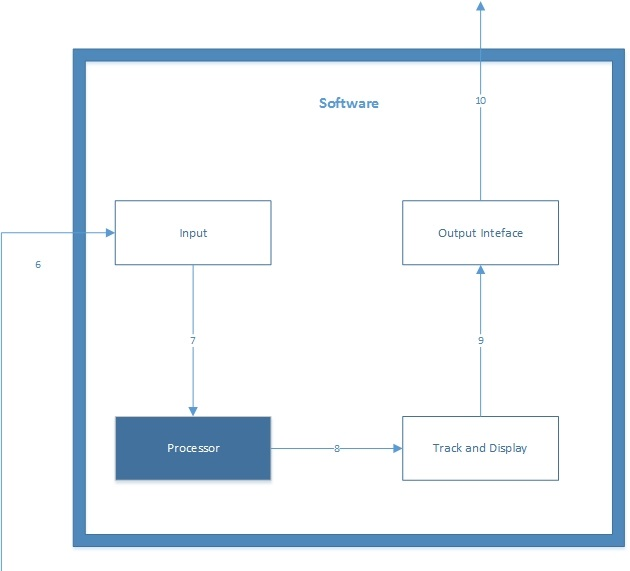
\includegraphics[width=0.60\textwidth]{images/Software_Processor.jpg}
 \caption{Processor Subsystem}
\end{figure}



\subsubsection{Assumptions}
%Any assumptions made in the definition of the subsystem should be listed and described. Pay particular attention to assumptions concerning interfaces and interactions with other layers.
We assume that we are getting video data from the Input Subsystem at 30 frames per second. 

%Repeat for each subsystem
\subsubsection{Responsibilities}
%Each of the responsibilities/features/functions/services of the subsystem as identified in the architectural summary must be expanded to more detailed responsibilities. These responsibilities form the basis for the identification of the finer-grained responsibilities of the layer's internal subsystems. Clearly describe what each subsystem does.
The processor is responsible for utilizing various computer vision algorithms to properly track the pupil. First, the processor needs to smooth each frame in the video. Next, it needs to apply the canny edge detector
to detect all the edges. Finally, this processor sends all the detected edges to the Track and Display subsystem. 

\subsubsection{Subsystem Interfaces}
%Each of the inputs and outputs for the subsystem are defined here. Create a table with an entry for each labelled interface that connects to this subsystem. For each entry, describe any incoming and outgoing data elements will pass through this interface.
This subsystem gets input of video data and output of a somewhat refined video data.

\begin {table}[H]
\caption {Processor Subsystem Interface} 
\begin{center}
    \begin{tabular}{ | p{1cm} | p{6cm} | p{3cm} | p{3cm} |}
    \hline
    ID & Description & Inputs & Outputs \\ \hline
    \#07 & Process Video Frames & \pbox{3cm}{Video Data} & \pbox{3cm}{ Detected Edges }  \\ \hline
    %\#xx & Description of the interface/bus & \pbox{3cm}{N/A} & \pbox{3cm}{output 1}  \\ \hline
    \end{tabular}
\end{center}
\end{table}
\newline

\subsection{Track and Display Subsystem}
This subsystem receives some video data whose edges have been detected by the processor subsytem and it tracks and displays the results. 

\begin{figure}[h!]
	\centering
 	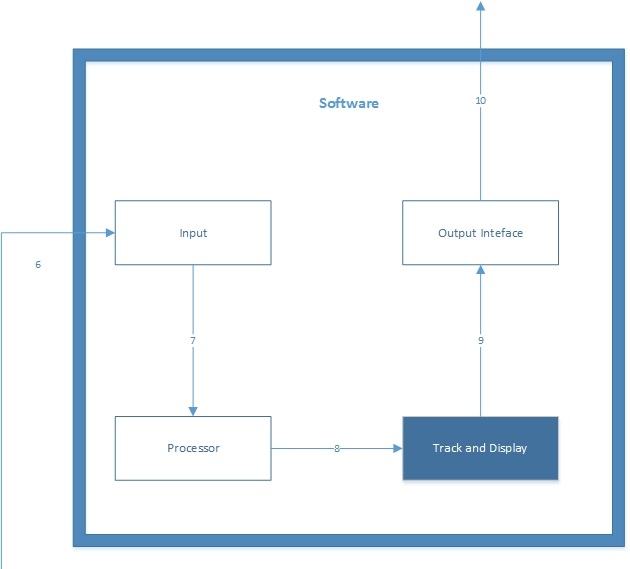
\includegraphics[width=0.60\textwidth]{images/Software_Track.jpg}
 \caption{Tracker Subsystem}
\end{figure}

\subsubsection{Assumptions}
%Any assumptions made in the definition of the subsystem should be listed and described. Pay particular attention to assumptions concerning interfaces and interactions with other layers.
We assume that this subsystem recieves frames whos edges have been detected. 

%Repeat for each subsystem
\subsubsection{Responsibilities}
%Each of the responsibilities/features/functions/services of the subsystem as identified in the architectural summary must be expanded to more detailed responsibilities. These responsibilities form the basis for the identification of the finer-grained responsibilities of the layer's internal subsystems. Clearly describe what each subsystem does.
This subsystem is responsible for applying the pupil tracking algorithm to the input it receives. It then applies the RANSAC algorithm to fit an ellipse to the pupil. Finally, it
displays the video with tracked pupil. 

\subsubsection{Subsystem Interfaces}
%Each of the inputs and outputs for the subsystem are defined here. Create a table with an entry for each labelled interface that connects to this subsystem. For each entry, describe any incoming and outgoing data elements will pass through this interface.
This subsystem receives edges that were detected by the processing subsystem and outputs the final results in a video stream. 

\begin {table}[H]
\caption {Track and Display Subsystem interface} 
\begin{center}
    \begin{tabular}{ | p{1cm} | p{6cm} | p{3cm} | p{3cm} |}
    \hline
    ID & Description & Inputs & Outputs \\ \hline
    \#08 & Receive data and display & \pbox{3cm}{Detected Edges } & \pbox{3cm}{Tracked Eye}  \\ \hline
    %\#xx & Description of the interface/bus & \pbox{3cm}{N/A} & \pbox{3cm}{output 1}  \\ \hline
    \end{tabular}
\end{center}
\end{table}
\newline

\subsection{Output Subsystem}
This subsystem simply provides an interface to send a video stream to some external device or module via ethernet or USB. The exeternal device or module shall be either a computer monitor or a cell phone or a webpage. 


\begin{figure}[h!]
	\centering
 	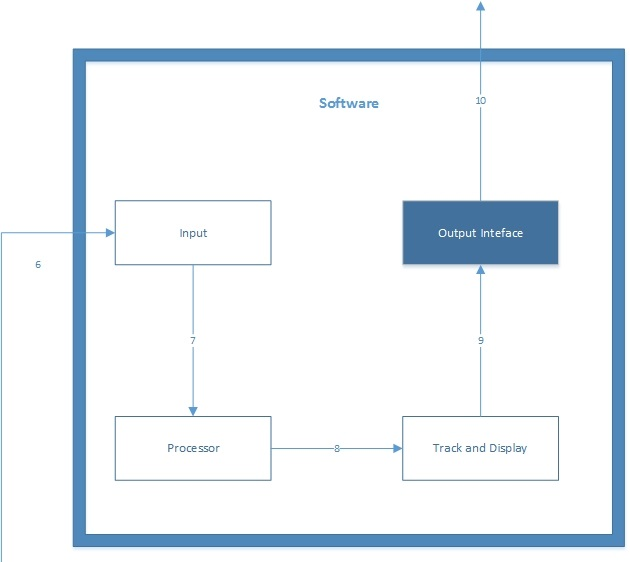
\includegraphics[width=0.60\textwidth]{images/Software_Output.jpg}
 \caption{Output Subsystem}
\end{figure}

\subsubsection{Assumptions}
%Any assumptions made in the definition of the subsystem should be listed and described. Pay particular attention to assumptions concerning interfaces and interactions with other layers.
We assume that this subsystem recieves video frames that show the tracked pupil. 

%Repeat for each subsystem
\subsubsection{Responsibilities}
%Each of the responsibilities/features/functions/services of the subsystem as identified in the architectural summary must be expanded to more detailed responsibilities. These responsibilities form the basis for the identification of the finer-grained responsibilities of the layer's internal subsystems. Clearly describe what each subsystem does.
This subsystem is responsible for properly sending the final result (video) of the entire system to an output device such a computer monitor. 

\subsubsection{Subsystem Interfaces}
%Each of the inputs and outputs for the subsystem are defined here. Create a table with an entry for each labelled interface that connects to this subsystem. For each entry, describe any incoming and outgoing data elements will pass through this interface.
This subsystem receives videos and provides an interface for an output device such as a monitor.  

\begin {table}[H]
\caption {Output Subsystem Interface} 
\begin{center}
    \begin{tabular}{ | p{1cm} | p{6cm} | p{3cm} | p{3cm} |}
    \hline
    ID & Description & Inputs & Outputs \\ \hline
    \#09 & Send video data to external device & \pbox{3cm}{Tracked Eye } & \pbox{3cm}{Tracked Eye}  \\ \hline
    %\#xx & Description of the interface/bus & \pbox{3cm}{N/A} & \pbox{3cm}{output 1}  \\ \hline
    \end{tabular}
\end{center}
\end{table}




\newpage

%%% References
\bibliographystyle{plain}
\bibliographystyle{reference/IEEEtran_custom}
\bibliography{reference/refs}{}

\end{document}